\subsection{Kiến trúc tổng thể}
Hệ thống gồm \textbf{hai khối tách rời về mặt vật lý} (Hình 3.1), đúng theo mục tiêu ``người vận hành đứng ngoài vùng nguy hiểm'' đã nêu ở mục 1.1.

\begin{figure}[!htbp]
  \centering
  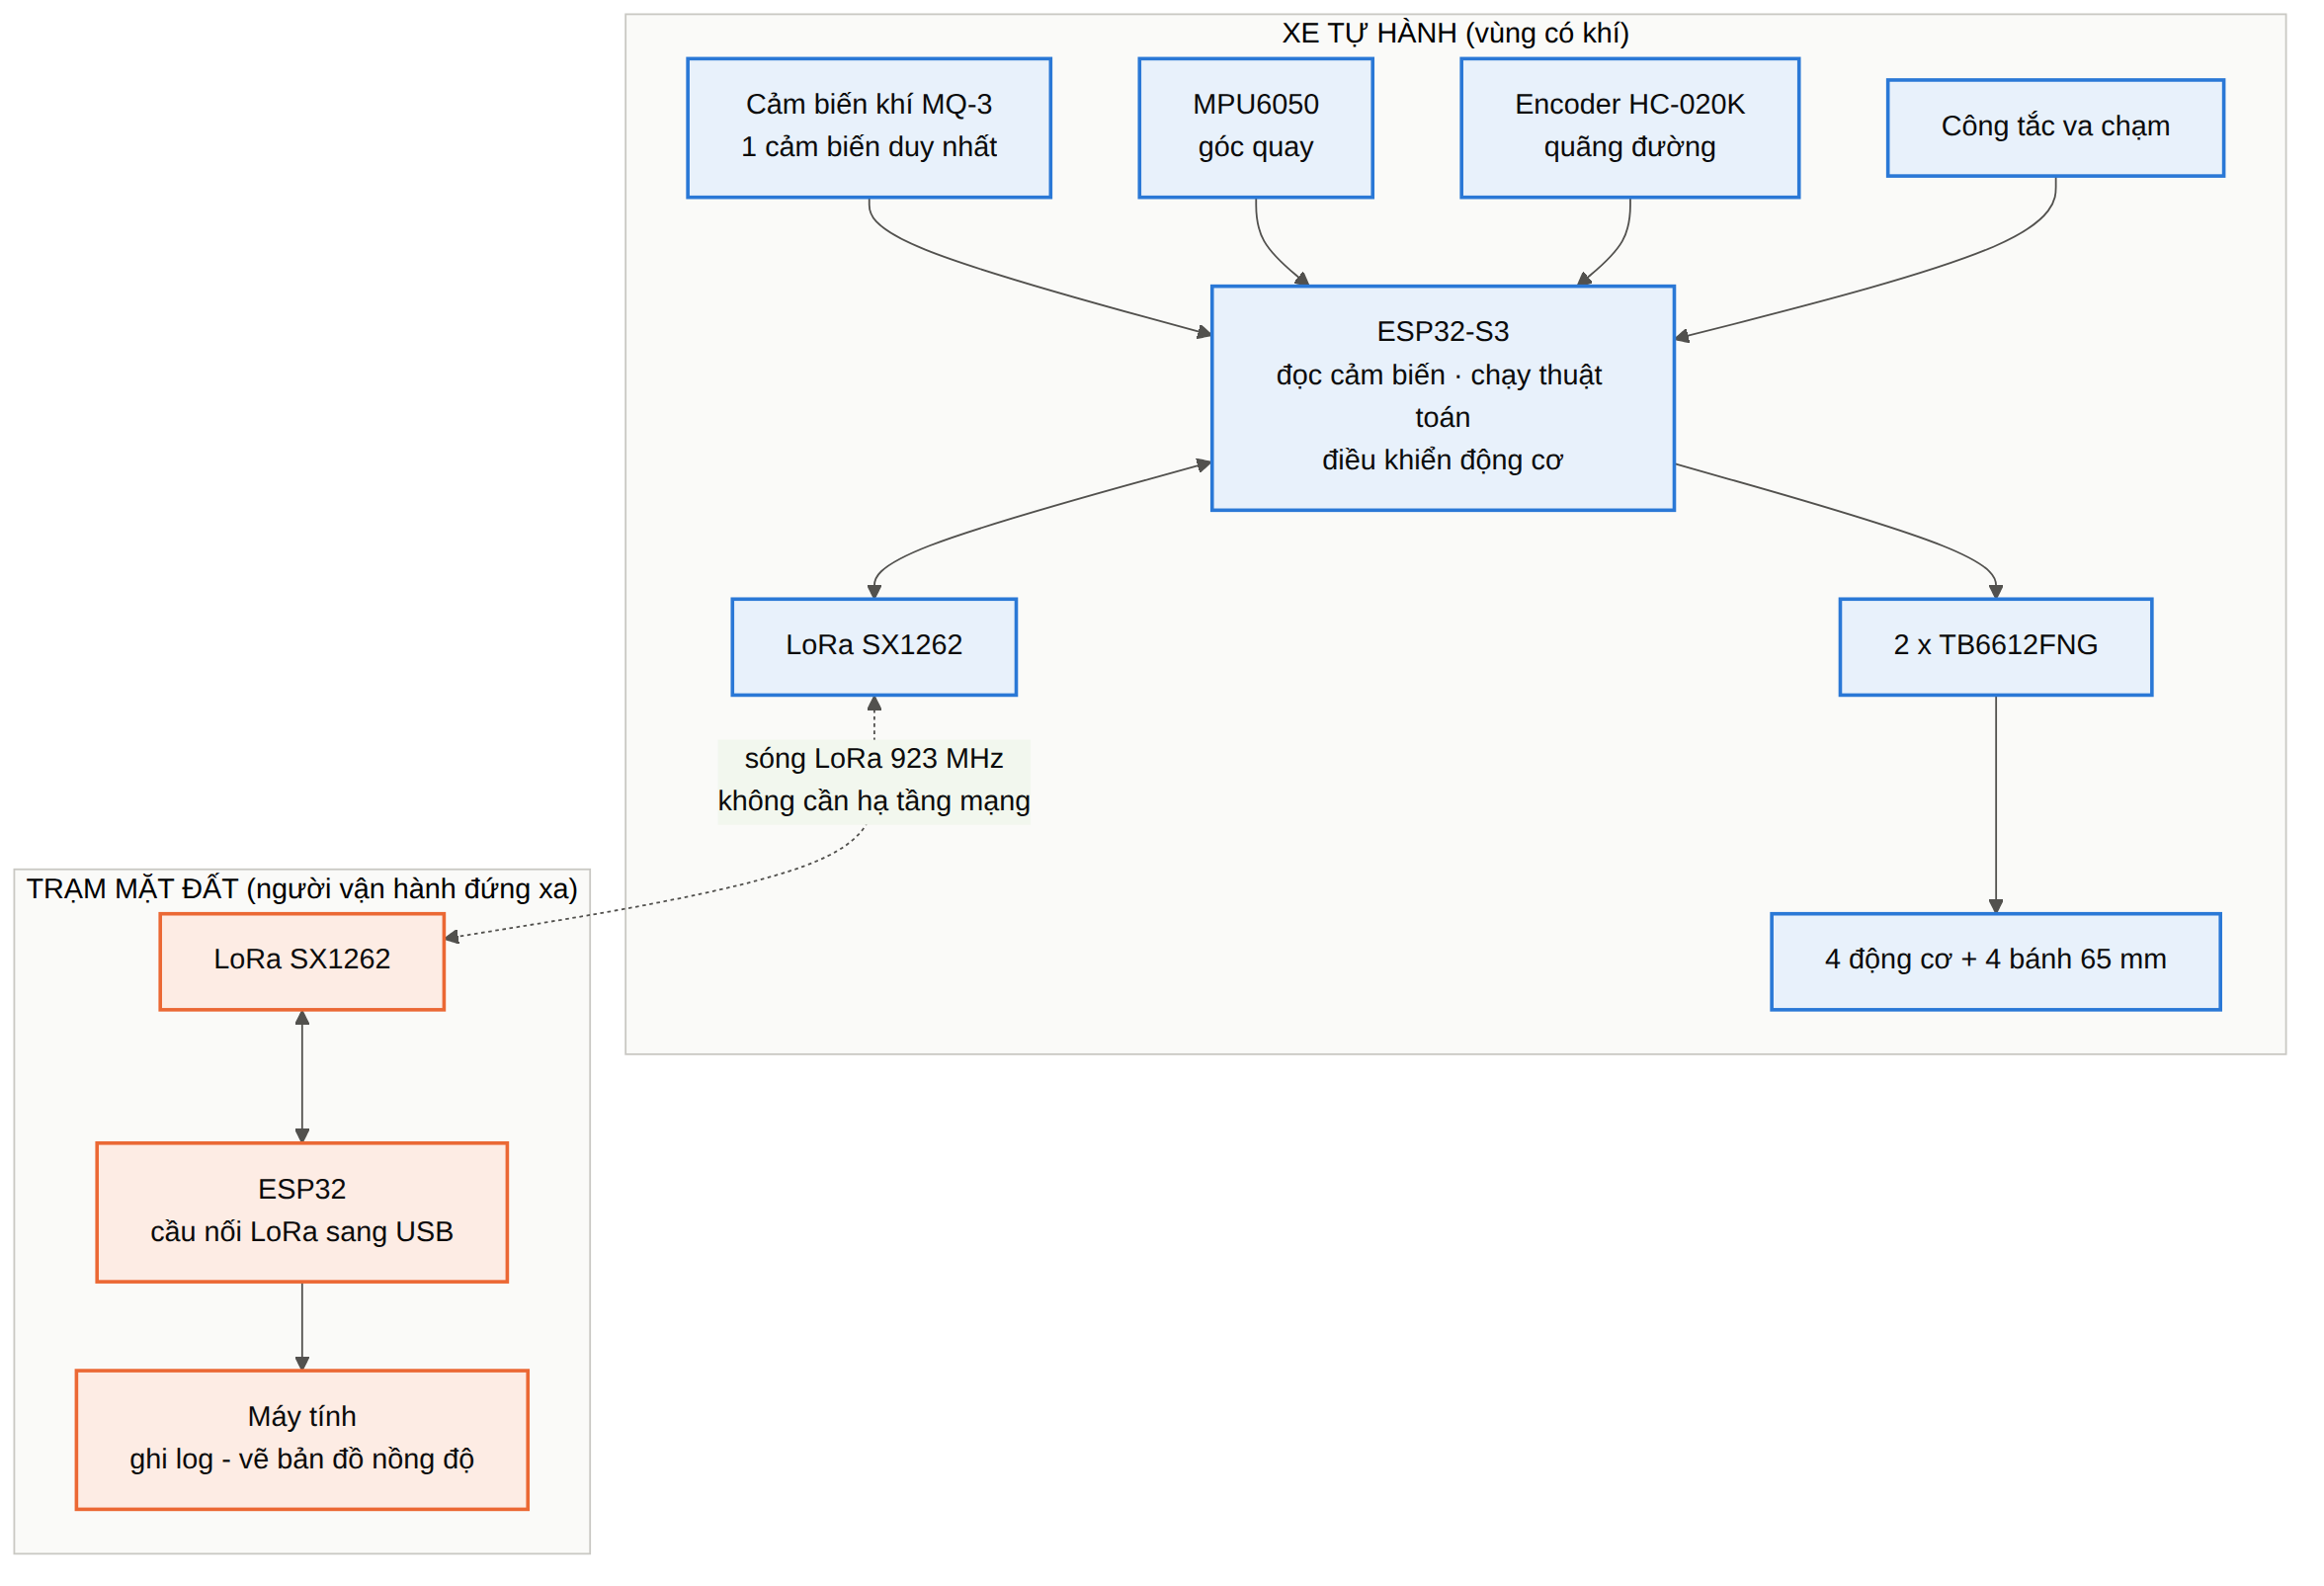
\includegraphics[width=0.941\textwidth]{pic/1_so_do_khoi.png}
  \caption{Sơ đồ khối hệ thống GasSeeker. Khối bên trái hoạt động trong vùng có khí; khối bên phải nằm ở vị trí an toàn, nối với nhau chỉ bằng một đường truyền LoRa.}
\end{figure}
\textbf{Khối thứ nhất là xe tự hành}, hoạt động trong vùng có khí. Trên xe có: một cảm biến khí MQ-3; một cảm biến gia tốc -- con quay MPU6050 để đo góc quay; một encoder quang HC-020K để đo quãng đường; một công tắc va chạm ở đầu xe; bốn động cơ điều khiển qua hai mạch cầu H; và một module LoRa. Bộ xử lý trung tâm là một ESP32-S3: nó đọc cảm biến, chạy thuật toán tìm nguồn và ra lệnh cho động cơ.

\textbf{Khối thứ hai là trạm mặt đất}, nơi người vận hành đứng. Trạm gồm một module LoRa và một ESP32 thứ hai làm cầu nối, đưa dữ liệu về máy tính để ghi log và vẽ lại hành trình.

\begin{ghichu}
\textbf{Vì sao cần đến hai vi điều khiển?} Đây không phải hai vi điều khiển trên cùng một xe, mà là \textbf{hai đầu của một đường truyền}. Mục tiêu của đề tài là người vận hành không phải đi vào vùng có khí, nên bắt buộc phải có truyền không dây, mà một đường truyền thì phải có hai đầu. Module LoRa SX1262 giao tiếp qua SPI nên không cắm thẳng vào máy tính được; đầu thu vì vậy cần một vi điều khiển làm cầu nối SPI sang USB. Bỏ nó đi thì không mất một tính năng phụ nào cả --- mất luôn khả năng giám sát từ xa, tức là mất mục tiêu chính của đề tài.
\end{ghichu}
\begin{ghichu}
\textbf{Vì sao dùng LoRa mà không dùng Wi-Fi có sẵn trên ESP32?} Hai lý do. Thứ nhất là hạ tầng: LoRa đạt cự ly hàng trăm mét mà \textbf{không cần một điểm phát sóng nào}, còn Wi-Fi thì cần một access point phủ tới đúng chỗ đang rò rỉ --- trong nhà xưởng hay bãi rác thì thường là không có. Thứ hai là nhiễu nội bộ: trên ESP32, khối Wi-Fi dùng chung tài nguyên với bộ chuyển đổi ADC2, nên bật Wi-Fi sẽ làm việc lấy mẫu tín hiệu khí kém ổn định. Nhóm muốn giữ đường đọc cảm biến khí sạch nhất có thể, vì đó là tín hiệu quyết định cả bài toán.
\end{ghichu}

\subsection{Lựa chọn linh kiện}
Mọi linh kiện đều được chọn theo một nguyên tắc chung: \textbf{giữ đường đọc tín hiệu khí sạch nhất có thể}, và không chi tiền vào những chỗ không làm thay đổi kết luận của đề tài. Bảng 3.1 liệt kê các linh kiện chính kèm lý do lựa chọn; ba mục đáng chú ý nhất --- vi điều khiển, cảm biến khí và module truyền tin --- được phân tích kỹ hơn ngay sau bảng và ở các mục 2.2.4, 3.3 và 3.6.

\begin{table}[!htbp]
  \centering
  \caption{Danh mục linh kiện chính và lý do lựa chọn}
  \small
  \renewcommand{\arraystretch}{1.25}
  \begin{tabular}{>{\raggedright\arraybackslash}p{0.1806\textwidth}>{\raggedright\arraybackslash}p{0.1987\textwidth}>{\raggedright\arraybackslash}p{0.5239\textwidth}}
    \toprule
    \textbf{Khối} & \textbf{Linh kiện} & \textbf{Lý do lựa chọn} \\
    \midrule
    Vi điều khiển & ESP32-S3 DevKitC-1 & ADC 12 bit (so với 10 bit của nhiều dòng 8 bit) là yếu tố quyết định, vì bài toán dựa trên việc phân biệt các chênh lệch nhỏ của tín hiệu khí; ngoài ra có đủ chân, đủ tốc độ và hỗ trợ SPI cho LoRa \\
    Cảm biến khí & MQ-3 & Rẻ, đọc được hơi cồn, có datasheet đầy đủ; độ chính xác thấp không ảnh hưởng kết luận vì thuật toán chỉ dùng tín hiệu tương đối (xem mục 2.2.4) \\
    Cảm biến hướng & MPU6050 / GY-521 & Cung cấp tốc độ góc quanh trục đứng; \textbf{bắt buộc} trong cấu hình một encoder vì không thể suy góc quay từ hiệu hai encoder \\
    Đo quãng đường & Encoder quang HC-020K, đĩa 20 khe & Một xung ứng với $\pi$$\cdot$65/20 $\approx$ 10,2 mm quãng đường --- đủ mịn cho bước đi 25--30 cm \\
    Động cơ và bánh & 4 động cơ giảm tốc V1, bánh 65 mm & Bốn bánh cho lực kéo ổn định trên mặt sàn phòng thí nghiệm \\
    Mạch cầu H & 2 $\times$ TB6612FNG & Mỗi động cơ nằm trên một cầu H riêng; hiệu suất cao hơn và sụt áp thấp hơn L298N \\
    Va chạm & 1 công tắc hành trình V156 & Phản ứng va chạm là mức tối thiểu cần thiết; đề tài không đặt mục tiêu né vật cản \\
    Truyền tin & SX1262 / Ra-01SH & Cự ly xa, không cần hạ tầng; băng 923 MHz nằm trong băng SRD của Việt Nam \\
    Nguồn & 2 $\times$ pin 18650 nối tiếp, XL4015 + LM2596 & Hai nhánh hạ áp độc lập (xem mục 3.3) \\
    \bottomrule
  \end{tabular}
\end{table}

\subsection{Thiết kế mạch nguồn}
\begin{figure}[!htbp]
  \centering
  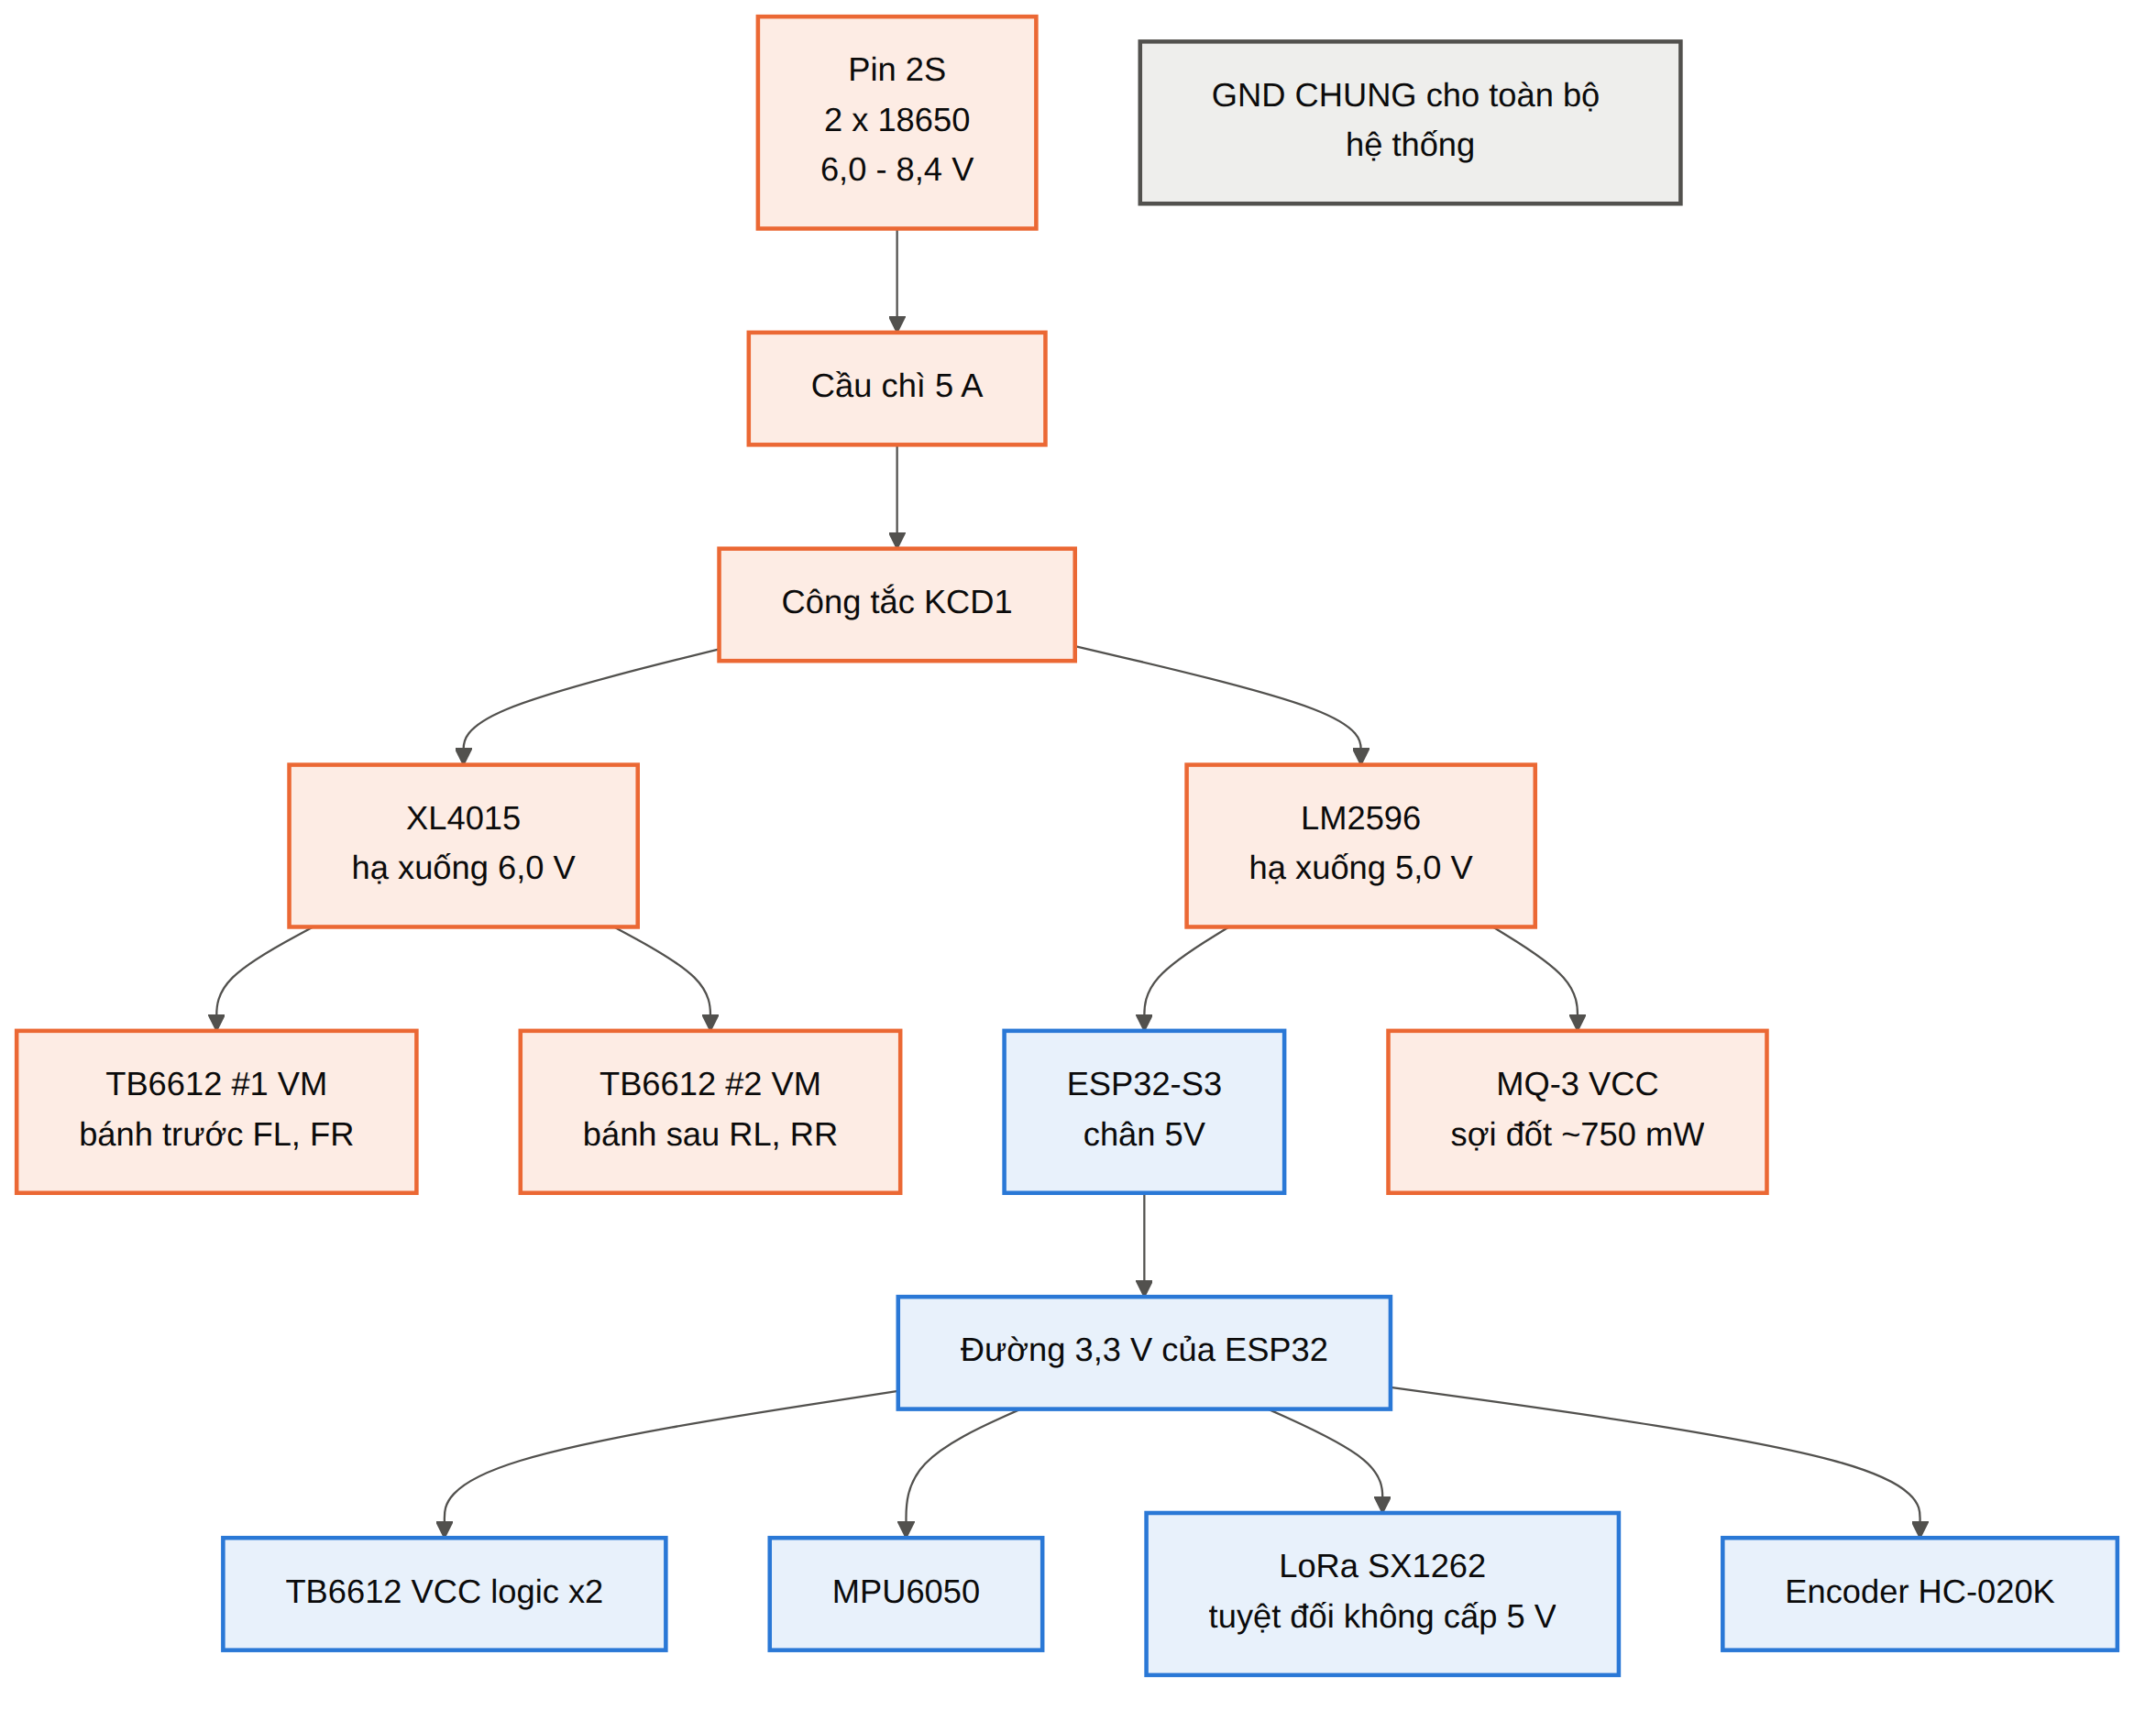
\includegraphics[width=0.882\textwidth]{pic/2_so_do_nguon.png}
  \caption{Sơ đồ phân phối nguồn. Nhánh động cơ và nhánh cảm biến tách nhau ngay từ pin, mỗi nhánh có mạch hạ áp riêng.}
\end{figure}
Hình 3.2 mô tả toàn bộ đường phân phối nguồn. Nguồn là hai pin 18650 nối tiếp, cho điện áp 6,0 tới 8,4 V tuỳ trạng thái sạc. Ngay sau cực dương là \textbf{cầu chì 5 A} rồi \textbf{công tắc chính KCD1}. Từ đó nguồn tách làm hai nhánh:

\begin{itemize}[leftmargin=1.4em,itemsep=0.15em,topsep=0.3em]
  \item Mạch hạ áp \textbf{XL4015} đưa xuống \textbf{6,0 V}, cấp cho chân VM của hai mạch cầu H điều khiển động cơ.
  \item Mạch hạ áp \textbf{LM2596} đưa xuống \textbf{5,0 V}, cấp cho ESP32 và cho sợi đốt của cảm biến MQ-3.
\end{itemize}
Đường \textbf{3,3 V} lấy ra từ bộ ổn áp trên board ESP32 nuôi toàn bộ phần logic: chân VCC của hai mạch cầu H, MPU6050, module LoRa và encoder.

Ba nguyên tắc thiết kế được tuân thủ chặt chẽ:

\textbf{Thứ nhất, tách nhánh động cơ khỏi nhánh cảm biến ngay từ pin.} Động cơ là tải đóng cắt liên tục; nếu dùng chung một mạch hạ áp với cảm biến thì mỗi lần xe khởi động hay đảo chiều, điện áp sẽ sụt và giá trị đọc từ cảm biến khí sẽ nhảy theo. Nghiêm trọng hơn, sụt áp làm \textbf{sợi đốt của MQ-3 hạ nhiệt}, và điện trở lớp nhạy khí phụ thuộc trực tiếp vào nhiệt độ sợi đốt. Hệ quả là một \textbf{tương quan giả} giữa chuyển động của xe và giá trị nồng độ đọc được --- đúng loại nhiễu nguy hiểm nhất cho một đề tài mà toàn bộ kết luận dựa trên việc so sánh những chênh lệch nhỏ của tín hiệu khí.

\textbf{Thứ hai, module LoRa chỉ được cấp 3,3 V}, tuyệt đối không cấp 5 V, và phải gắn ăng-ten trước khi cấp nguồn để tránh hỏng tầng khuếch đại công suất.

\textbf{Thứ ba, chân đọc tín hiệu MQ-3 đi qua một mạch chia áp 10 k$\Omega$ / 20 k$\Omega$}, vì đầu ra tương tự của MQ-3 có thể lên tới gần 5 V trong khi chân ESP32 chỉ chịu được 3,3 V. Hệ số chia là 20/(10 + 20) = 0,667; hệ số này nằm trong firmware để tính ngược lại điện áp thật tại chân AO.

Ngoài ra, các tụ chống nhiễu được lắp theo nguyên tắc: 100 nF trực tiếp qua hai cực \textbf{mỗi động cơ}; 470--1000 $\mu$F gần đường VM của hai mạch cầu H; 220--470 $\mu$F gần ESP32; 220--470 $\mu$F kèm 100 nF sát chân nguồn LoRa; và 100 nF từ chân đọc MQ-3 xuống GND.


\subsection{Sơ đồ đấu nối và phân bổ chân}
\begin{figure}[!htbp]
  \centering
  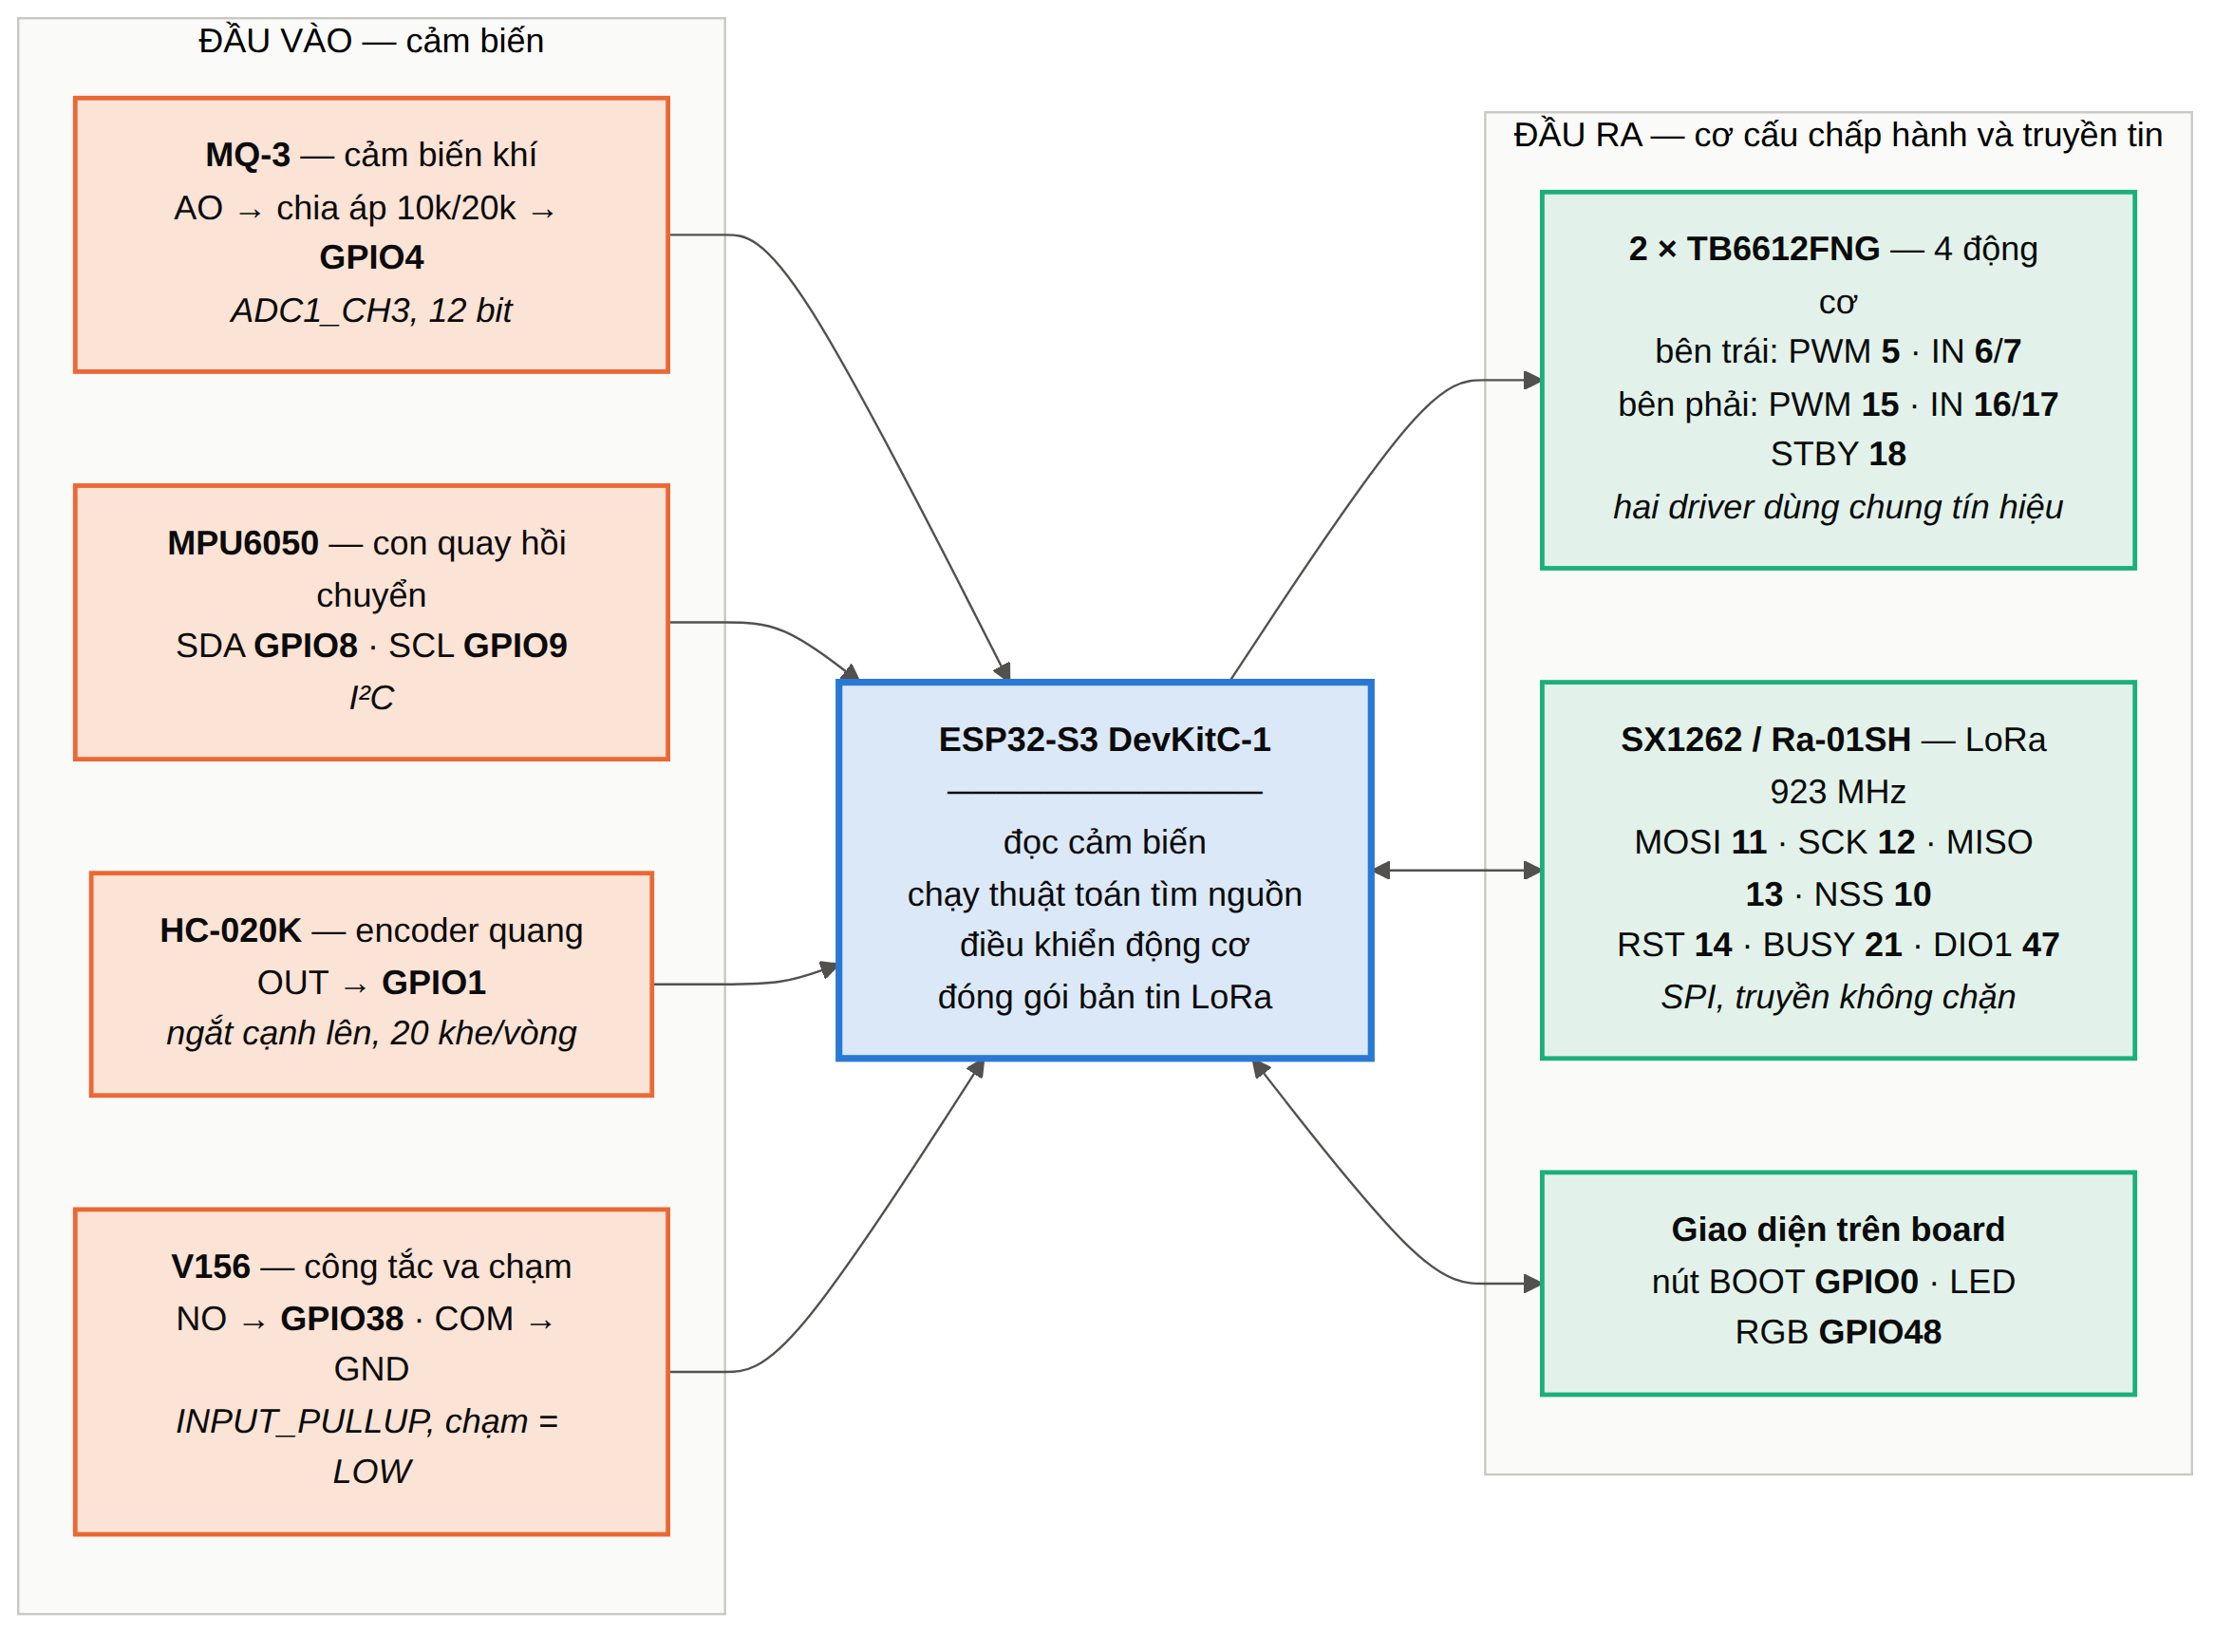
\includegraphics[width=0.941\textwidth]{pic/10_so_do_dau_noi.png}
  \caption{Sơ đồ đấu nối tổng thể và phân bổ chân GPIO trên ESP32-S3.}
\end{figure}
\begin{table}[!htbp]
  \centering
  \caption{Phân bổ chân GPIO trên ESP32-S3 DevKitC-1}
  \small
  \renewcommand{\arraystretch}{1.25}
  \begin{tabular}{>{\raggedright\arraybackslash}p{0.1084\textwidth}>{\raggedright\arraybackslash}p{0.2981\textwidth}>{\raggedright\arraybackslash}p{0.4968\textwidth}}
    \toprule
    \textbf{GPIO} & \textbf{Thiết bị} & \textbf{Ghi chú} \\
    \midrule
    0 & Nút BOOT trên board & Nhấn ngắn: chạy/dừng $\cdot$ Nhấn giữ 0,8 s: đổi thuật toán \\
    1 & HC-020K OUT & Encoder duy nhất, ngắt cạnh lên \\
    4 & MQ-3 AO & Qua mạch chia áp 10k/20k $\cdot$ ADC1\_CH3 \\
    5, 6, 7 & TB6612 PWMA, AIN1, AIN2 & Điều khiển bên trái (cả hai driver) \\
    8, 9 & MPU6050 SDA, SCL & Giao tiếp I$^{2}$C \\
    10--14, 21, 47 & LoRa NSS, MOSI, SCK, MISO, RST, BUSY, DIO1 & Giao tiếp SPI \\
    15, 16, 17 & TB6612 PWMB, BIN1, BIN2 & Điều khiển bên phải (cả hai driver) \\
    18 & TB6612 STBY & Dùng chung cho cả hai driver $\cdot$ LOW = tắt động cơ \\
    38 & Công tắc va chạm & INPUT\_PULLUP $\cdot$ chạm = mức thấp \\
    48 & LED RGB trên board & Hiển thị bốn mức cảnh báo \\
    \bottomrule
  \end{tabular}
\end{table}
Hình 3.3 tổng hợp toàn bộ đường tín hiệu giữa vi điều khiển và các khối ngoại vi, còn Bảng 3.2 liệt kê chi tiết từng chân. Ba nhóm chân sau \textbf{được tránh hoàn toàn} vì lý do phần cứng: GPIO 3, 45, 46 là chân strapping quyết định cách khởi động; GPIO 19, 20 là USB D-- / D+; GPIO 26--32 dành cho SPI flash trong và GPIO 33--37 dành cho PSRAM octal trên phiên bản N16R8. Đây là một lỗi rất hay gặp và rất khó tìm ra khi đã lắp xong, nên nhóm rà soát ngay từ khâu thiết kế.

Hai đặc điểm của cấu hình phần cứng thực tế cần được ghi nhận rõ, vì chúng có tác động trực tiếp lên phần mềm:

\textbf{Bốn động cơ nhưng chỉ hai bộ tín hiệu điều khiển.} Hai mạch TB6612 nhận chung một bộ tín hiệu logic từ ESP32: bên trái dùng GPIO 5/6/7 cho cả bánh trước trái và bánh sau trái, bên phải dùng GPIO 15/16/17 cho hai bánh phải. Về mặt điều khiển, xe vẫn là \textbf{xe vi sai hai bên}, nên phần mềm không phải thay đổi gì. Mỗi động cơ vẫn nằm trên một cầu H riêng để không quá tải một kênh.

\textbf{Chỉ có một encoder, lắp ở bánh sau trái.} Đây là điểm khác biệt so với thiết kế ban đầu và nếu để nguyên sẽ gây hai lỗi nghiêm trọng: (i) công thức quãng đường trung bình hai bánh \textit{d} = (\textit{d}\textsubscript{L} + \textit{d}\textsubscript{R})/2 với \textit{d}\textsubscript{R} luôn bằng không sẽ làm \textbf{quãng đường bị tính xấp xỉ một nửa}; và (ii) khi quay tại chỗ, bánh trái vẫn quay nên robot sẽ \textbf{tưởng mình vừa đi lùi một đoạn}. Cách xử lý trong firmware được trình bày ở mục 4.1.


\subsection{Bố trí cơ khí và vị trí đặt cảm biến}
Cảm biến MQ-3 được gắn \textbf{lệch hẳn về phía trước xe}, cách tâm trục hai bánh khoảng \textbf{12 cm}. Đây không phải một chi tiết thẩm mỹ mà là một yêu cầu chức năng: nhờ khoảng lệch này, việc \textbf{quay tại chỗ cũng làm đầu dò đổi vị trí trong không gian}, và thao tác quét ba hướng của thuật toán bám gradient mới lấy được thông tin không gian. Nếu gắn cảm biến ngay tại tâm trục, quay tại chỗ không làm đầu dò di chuyển và thao tác quét ba hướng trở nên vô nghĩa.

Cụ thể, với góc quét $\pm$55$^\circ$, khoảng cách giữa hai vị trí đầu dò ở hai đầu quét là:

\[ 2 \times 12 \times \sin 55^{\circ} \approx 19{,}7~\text{cm} \approx 20~\text{cm} \]
Đây là một khoảng cách đo hiệu dụng có ý nghĩa, và nó lý giải vì sao giá trị 55$^\circ$ được chọn thay vì một góc nhỏ hơn.

MPU6050 được gắn phẳng và cố định chắc chắn trên khung, tương đối gần tâm xe, tránh đặt sát động cơ hoặc trực tiếp trên mạch cầu H và mạch hạ áp. Sau khi lắp, tư thế của module không được thay đổi giữa các lần hiệu chuẩn. Dây tín hiệu (MQ-3 AO, encoder OUT, I$^{2}$C, SPI, bumper) được đi tách khỏi bó dây công suất (pin, cầu chì, mạch hạ áp, dây động cơ).


\subsection{Đường truyền LoRa}
\begin{table}[!htbp]
  \centering
  \caption{Tham số cấu hình đường truyền LoRa}
  \small
  \renewcommand{\arraystretch}{1.25}
  \begin{tabular}{>{\raggedright\arraybackslash}p{0.3613\textwidth}>{\raggedright\arraybackslash}p{0.2258\textwidth}>{\raggedright\arraybackslash}p{0.3161\textwidth}}
    \toprule
    \textbf{Tham số} & \textbf{Giá trị} & \textbf{Ghi chú} \\
    \midrule
    Tần số & 923,0 MHz & Nằm giữa băng SRD Việt Nam 920--925 MHz \\
    Băng thông & 125 kHz & Cân bằng giữa tốc độ và độ nhạy \\
    Hệ số trải phổ (SF) & 9 & Dự phòng cự ly; hạ xuống SF7 nếu cần gói tin nhanh hơn \\
    Tỉ lệ mã sửa lỗi & 4/5 &  \\
    Công suất phát & 14 dBm & Tương đương 25 mW EIRP, đúng giới hạn cho phép \\
    Từ đồng bộ & 0x34 & Tách mạng riêng của nhóm \\
    Chu kỳ gửi telemetry & 1 Hz &  \\
    \bottomrule
  \end{tabular}
\end{table}
Bảng 3.3 tóm tắt cấu hình đường truyền. Một quyết định thiết kế quan trọng: \textbf{việc truyền LoRa được thực hiện không chặn}. Hàm truyền dạng chặn của thư viện RadioLib giữ chương trình khoảng 200 ms ở SF9; với tốc độ xe 18 cm/s, xe sẽ đi lố khoảng 3,6 cm cho mỗi gói tin --- đủ để làm sai lệch vị trí gắn với phép đo. Firmware vì vậy dùng cơ chế bắt đầu truyền rồi chờ cờ ngắt DIO1, để vòng điều khiển không bao giờ bị chặn.

Gói tin được gửi dưới dạng CSV kèm mã kiểm tra XOR theo kiểu NMEA, cho phép trạm thu phát hiện gói hỏng. Trạm in ra \textbf{cả hai dạng}: một dòng máy đọc để ghi log tự động và một dòng người đọc để theo dõi trực tiếp.

Cuối cùng, cần nhấn mạnh một nguyên tắc kiến trúc: \textbf{robot phải chạy được hoàn toàn khi mất LoRa}. Đường truyền chỉ phục vụ giám sát và dừng khẩn từ xa; toàn bộ logic ra quyết định nằm trên xe.
